\lvli{Introduction}

In this experiment we analyzed the behavior of an FBG (Fiber Bragg Grating). The FBG uses the Bragg Mirror, which is a specific type of photonic crystal that acts as a mirror for a given range of frequencies. This photonic crystall can be modeled as a multilayer film where two materials with different refractive index are alternated.Imagining an ideal Bragg mirror the reflected wavelength is defined as $\lambda_{BRAGG} = \frac{2\pi}{k_{BRAGG}}$ where $k_{BRAGG}$ it is the propagation constant of the phase and respects this rule $k_{BRAGG} \cdot (L_1 + L_2) = m \cdot \pi$ with $m \in \mathbb{N}$ and $L_1, L_2$ are the two lengths of the films. By inserting a Bragg mirror into the fiber we obtain a mechanical coupling between the two in particular in compression and elongation, in fact pulling the fiber is also pulled the mirror and then modified the period $(L_1 + L_2)$ which in turn changes $\lambda_{BRAGG}$. From this physical effect we can then relate elongation with the reflected frequency. This mirror, however, is also sensitive to temperature variations, in fact, in addition to creating an expansion or compression of the period, it introduces a variation of the silica refraction index induced by the thermo-optic effect.

The setup we use is composed of an optical amplifier that produces broadband light that is inserted into a fiber containing an FBG, the light that is reflected then passes through an optical circulator that sends it to a spectrum analyzer (Fig.\ref{fig:setup}).
\begin{figure}[h]
    \centering
    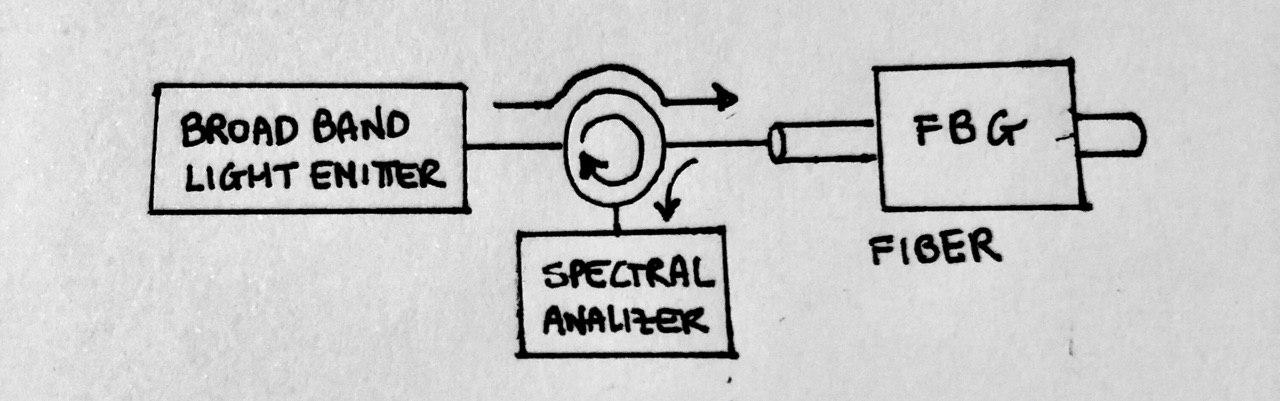
\includegraphics[scale=0.3]{img/setup.jpg}
    \caption{Setup.}
    \label{fig:setup}
\end{figure}

What is done in this experiment is to measure the reflected wave frequency according to the applied elongation. In this case the elongation is performed by turning a circular manual tensor (ring): each rotation corresponds to an elongation of $0.5 [mm]$ and on the ring there are 50 notches and therefore we have an elongation of $0.01 [mm] $for notch. Our fiber started from a length of $14 [mm]$ and we elongated it by $1.5 [mm]$. The measurements we have performed are shown in (Tab.\ref{table:measures}), where for each rotation the value of the reflected frequency calculated by eye was reported. The table has three measuring columns because more consecutive measurements have been made starting from $14 [mm]$ and reaching $14.75 [mm]$ then going back to $14 [mm]$ and then returning to $14.7 [mm] $. The table also specifies with $x$ the measurements where the spectrum was stored for computer analysis.
\begin{table}[h]
  \centering
  \begin{tabular}{c|c|c|c}
      Position [mm]  &  $\lambda_B$  [nm]  &  $\lambda_B$  [nm]  &  $\lambda_B$  [nm]  \\
      \hline
      14     &  1534,691     &  1534,682(x)  &  1534,682     \\
      14.05  &  1534.861     &  1534.87      &  1534.861     \\
      14.1   &  1535.032     &  1535.032     &  1535.041(x)  \\
      14.15  &  1535.229     &  1535.186     &  1535.212     \\
      14.2   &  1535.391     &  1535.357     &  1535.391(x)  \\
      14.25  &  1535.604(x)  &  1535.562(x)  &  1535.587     \\
      14.3   &  1535.784     &  1535.749     &  1535.767(x)  \\
      14.35  &  1535.937     &  1535.92      &  1535.946     \\
      14.4   &  1536.125     &  1536.108     &  1536.108(x)  \\
      14.45  &  1536.305     &  1536.262     &  1536.305     \\
      14.5   &  1536.509(x)  &  1536.45 (x)  &  1536.467(x)  \\
      14.55  &  1536.663     &  1536.646     &  1536.646     \\
      14.6   &  1536.851     &  1536.851     &  1536.842(x)  \\
      14.65  &  1537.03      &  1537.005     &  1537.005     \\
      14.7   &  1537.184     &  1537.184     &  1537.184(x)  \\
      14.75  &  1537.389(x)  &  1537.389     &  1537.38      \\

  \end{tabular}
  \caption{Measures.}
  \label{table:measures}
\end{table}
From a first analysis we obtain the curve shown in (Fig.\ref{fig:firstAnalisy}).
\begin{figure}[h]
    \centering
    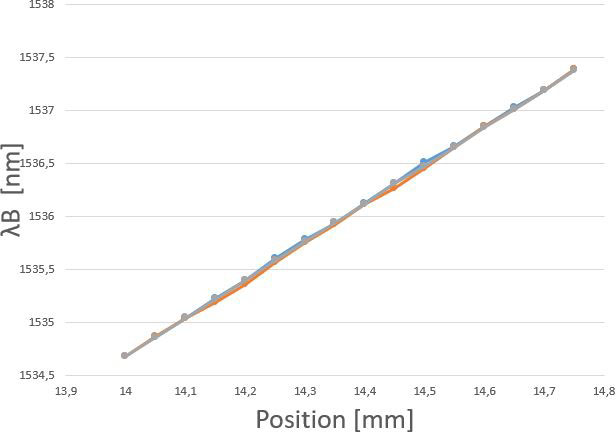
\includegraphics[scale=0.7]{img/firstAnalisy.jpg}
    \caption{First analisy.}
    \label{fig:firstAnalisy}
\end{figure}


\newpage
\lvli{Analysis}
First of all, the 13 files were imported. They contain the data related to the spectra measured by the spectrometer and contain: the two values of starting frequency and frequency step in THz; and then the list of reflected power values read in dB. The importation was made by converting the frequency values into wavelength values through the physical relation $\lambda = \frac{c_0}{f}$, to each of these values the corresponding power value has been assigned as shown in (Fig.\ref{fig:spectralPower}). From this figure it is also possible to clearly identify the peak to be analyzed, since while the signal has values lower than $-50[dB]$ and it has a value of approximately $-30[dB]$.
\begin{figure}[h]
    \centering
    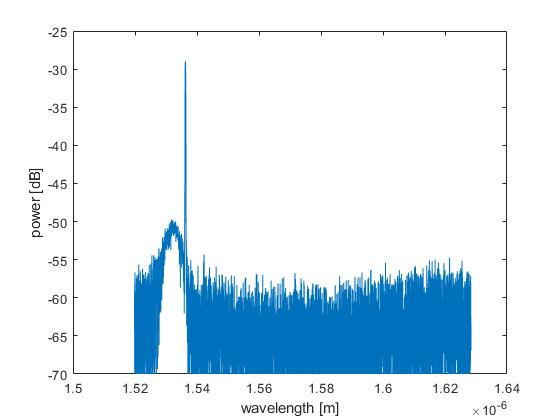
\includegraphics[scale=0.7]{img/spectralPower.jpg}
    \caption{Spectral power for 14[mm] of elongation.}
    \label{fig:spectralPower}
\end{figure}
At this point, for each file, the value of the wavelength corresponding to the maximum point is searched; to improve the analysis an interpolation of the points is performed through a quadratic function. A key point was to choose which points to consider in the approximation. The first attempt was through a classic approach, we chose to consider all the points that are above 90\% of the peak that resulted in a solution like in (Fig.\ref{fig:quadratic_fit_scale}), as you can see in this image there are a few 'points around the peak that add noise, the next choice would then be to opt for a greater percentage but doing so would have to calculate by hand for each spectrum the optimal value of percentage; instead another approach was chosen.
The alternative solution was based on the peak symmetry characteristic and follows the following approach: starting from the maximum point you move sideways until you find points with decreasing values, the example of filtering the points is shown in (Fig.\ref{fig:quadratic_fit}).

\begin{figure}[!htb]
  \minipage{0.32\textwidth}
    \centering
    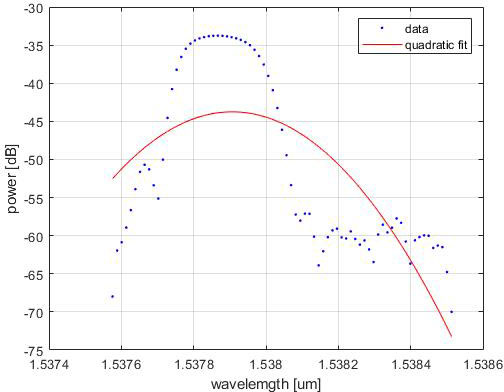
\includegraphics[scale=0.4]{img/quadratic_fit_scale_90.jpg}
    \caption{Quadratic fit scale 90\%.}
    \label{fig:quadratic_fit_scale}
  \endminipage\hfill
  \minipage{0.32\textwidth}
    \centering
    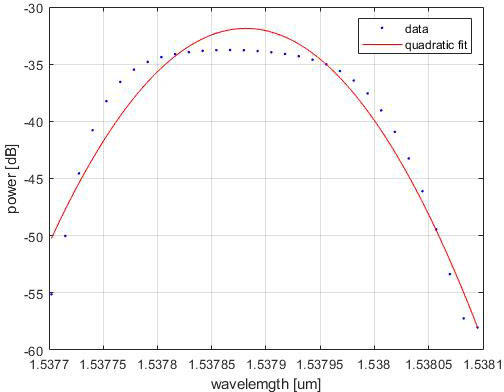
\includegraphics[scale=0.4]{img/quadratic_fit.jpg}
    \caption{Quadratic fit descending cutting mode.}
    \label{fig:quadratic_fit}
  \endminipage
\end{figure}

At this point it is put in relation to the values of the wavelengths newly computed with elongation values shown in (Fig.\ref{fig:spins}), having set the "14 [mm]" as our value of 0 we obtain an elongation of "0.75 [mm]". From here we proceeded with a linear fit to be able to derive the angular coefficient that corresponds to $a = \frac{\Delta \lambda}{\mu \epsilon} = 3.588 \cdot 10^{-3}$, it contains the information on the deformation of the FBG which depends on the temperature and the elongation.
\begin{figure}[h]
    \centering
    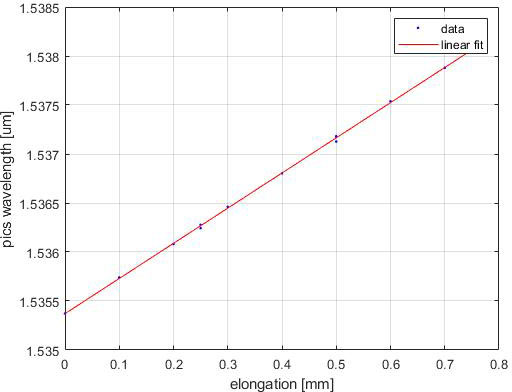
\includegraphics[scale=0.7]{img/spins.jpg}
    \caption{Elongation.}
    \label{fig:spins}
\end{figure}
 Assuming that the temperature inside the room was homogeneous and that we carried out the experiment in a sufficiently short time, the effect of temperature becomes negligible compared to that of elongation. This is also confirmed by the linear trend of the data obtained which is detached from the line of fit of only $RMSE = 1.6 \cdot 10^{-5}$. From this value we can calculate the sensitivity of the instrument using the formula:
$$s = \frac{L}{a} = 0.0865[\mu \epsilon]$$
with $L=310.5[mm]$ the length of the fiber at rest.


\newpage
\lvli{Conclusion}
The value obtained is very similar to the typical values for sensors of this type:
$$\Delta(\mu\epsilon) = \frac{1 [pm]}{ 1.2 [\frac{pm}{\mu\epsilon}]} \approx 0.8 [\mu \epsilon]$$
The performance of the data collected was excellent because they produced a linear trend as we expected with a deviation of $RMSE = 1.6 \cdot 10^{-5}$. Having performed both contraction and elongation measurements, we have had the possibility to check the existence or absence of a hysteresis behavior. Data collected although very few suggest lack of hysteresis given the low value of RMSE.

%% DOMANDE PROF
% 1) ho un fattore 10 che non mi torna
% 2) c'è qualche modo in cui possa ricavarmi l'incertezza sulla sensibility?
% 3) c'è altro che si può aggiungere?
% 4) lo spettometro legge potenza? in dB?
